\documentclass{beamer}
\mode<presentation>
\usetheme{CambridgeUS}
\usepackage[russian]{babel}
\usepackage[utf8]{inputenc}
\usepackage[T2A]{fontenc}
\usepackage{sansmathaccent}
\linespread{0.8}
\usepackage{verbatim}
\usepackage{alltt}

\pdfmapfile{+sansmathaccent.map}
\title[Artifical Intelligence]{Нейронные сети}
\author{Наумов Д.А., доц. каф. КТ}
\date[11.02.2019] {Экспертные системы и искусственный интеллект, 2019}

\begin{document}

%ТИТУЛЬНЫЙ СЛАЙД
\begin{frame}
  \titlepage
\end{frame}
  
%СОДЕРЖАНИЕ ЛЕКЦИИ
\begin{frame}
  \frametitle{Содержание лекции}
  \tableofcontents  
\end{frame}

\section{Математические основы нейронных сетей}

\begin{frame}[t]
	\begin{block}{Нейронные сети и нейрокомпьютеры}
		направление в компьютерной индустрии, в основе которого лежит идея создания искусственных интеллектуальных устройств по образу и подобию человеческого мозга.
	\end{block}
	\begin{figure}[h]
		\centering
		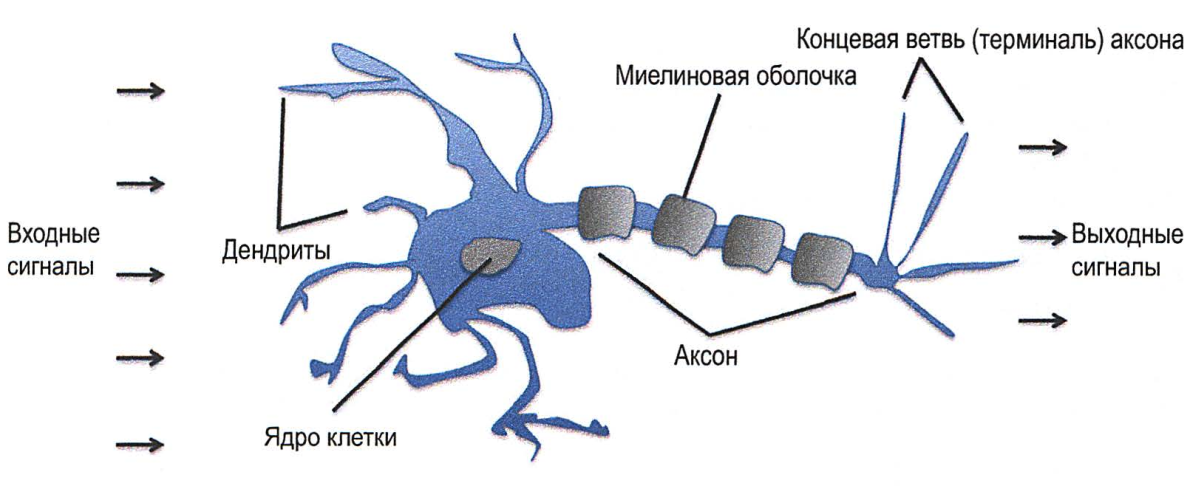
\includegraphics[scale=0.3]{images/lec03-pic01.png}
	\end{figure}
	Нейрон (у человека прилизительно $10^{11}$):
	\begin{itemize}
		\item получает информацию через дендриты (до $10^5$);
		\item передает информацию через аксон, разветвляющийся на синапсы (до $10^4$).
		\item может находиться в возбужденном и невозбужденном состоянии.		
	\end{itemize}
\end{frame}
	
\begin{frame}[t]{Модель нейрона}
	Гипотеза математического нейрона -– устройства, моделирующего нейрон мозга человека.
	\begin{figure}[h]
		\centering
		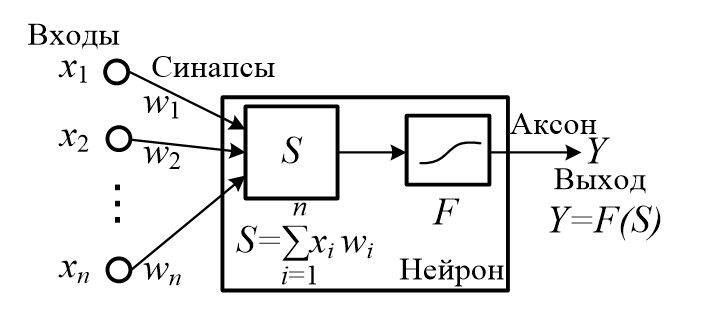
\includegraphics[scale=0.5]{images/lec03-neuron.png}
	\end{figure}
	\begin{enumerate}
		\item У. Маккалок и У. Питтс, <<Логическое исчисление идей, относящихся к нервной активности>>, Bulletin of Mathematical Biophysics (Бюллетень математической биофизики), 5 (4):115-133, 1943);
	\end{enumerate}
\end{frame}

\begin{frame}[t]{Модель нейрона}	
	Математический нейрон:
	\begin{itemize}
		\item имеет несколько входов, $N$ -- количество входов; 
		\item принимается входные сигналы $X=\{x_1, x_2,...,x_N\}=\{x_i\}, i=1..N$;
		\item суммирует входные сигналы, умножая их на весовой коэффициент $W=\{w_i\}, i=1..N$;
	\end{itemize}
	\[S=\sum_{i=1}^{N} x_i*w_i \]
	Выходной сигнал y может принимать одно из двух значений -- нуль или единица и формируется по следующему правилу:
	\[ y =
		\begin{cases}
		1 & \text{если } S\geq w_0 \\
		0 & \text{если } S< w_0
		\end{cases}
	\]
\end{frame}

\begin{frame}
	\linespread{1.0}
	Каждый нейрон:
	\begin{itemize}
		\item представляет собой пороговый элемент с несколькими входами и одним выходом;
		\item имеет свое определенное значение порога $w_0$;
		\item если взвешенная сумма входных сигналов не достигает порога чувствительности, то нейрон не возбужден и его выходной сигналe $y=0$;
		\item если же входные сигналы достаточно интенсивны и их сумма достигает порога чувствительности, то нейрон переходит в возбужденное состояние и на его выходе образуется сигнал $y=1$;
		\item весовые коэффициенты $w_i$ имитируют электропроводность нервных волокон -– силу синаптических связей между нейронами. 		
	\end{itemize}
	\linespread{0.8}	
\end{frame}

\begin{frame}
	\linespread{1.0}
	Логическая функция y(S) называется \textbf{активационной функцией}.
	\[ y =
		\begin{cases}
		1 & \text{если } S\geq w_0 \\
		0 & \text{если } S< w_0
		\end{cases}
	\]	
	\begin{figure}[h]
		\centering
		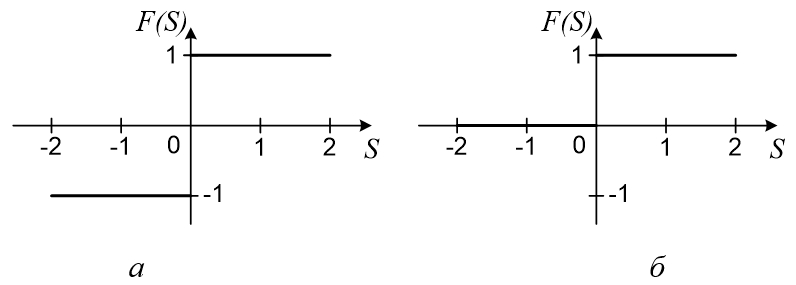
\includegraphics[scale=0.5]{images/lec03-activation.png}
	\end{figure}
	\begin{itemize}
		\item a - \textit{симметричная} активационная функция;
		\item б - \textit{смещенная} активационная функция.
	\end{itemize}
	\linespread{0.8}	
\end{frame}

\begin{frame}{Персептрон}
	\linespread{1.0}
	\begin{itemize}
		\item У. Мак-Каллок и В. Питтс высказали идею о том, что сеть из математических нейронов в состоянии обучаться, распознавать образы, обобщать, т.е. она обладает свойствами человеческого интеллекта.	
		\item Эта идея была материализована в 1958 году Фрэнком Розенблаттом сначала в виде компьютерной программы, а затем в виде электронного устройства, моделирующего человеческий глаз.
		\item Это устройство представляло собой совокупность искусственных нейронов Мак-Каллока – Питтса и было названо персептроном. 
		\item Устройство удалось обучить решению сложнейшей интеллектуальной задачи – распознаванию букв латинского алфавита.
	\end{itemize}		

	Ф. Розенблатт, <<Персептрон, воспринимающий и распознающий автомат>> Coгnell Aeronautical Laboratoгy (Лаборатория аэронавтики Корнелльского университета), 1957).
	\linespread{0.8}	
\end{frame}

\begin{frame}{Задача классификации цифр}
	\begin{itemize}
		\item \textbf{Задача}: классификация цифр на четные и нечетные.
		\item \textbf{Цель обучения персептрона}: чтобы $y=1$, если на карточке четная цифра, и $y=0$, если цифра нечетная.		
	\end{itemize}
	\begin{figure}[h]
		\centering
		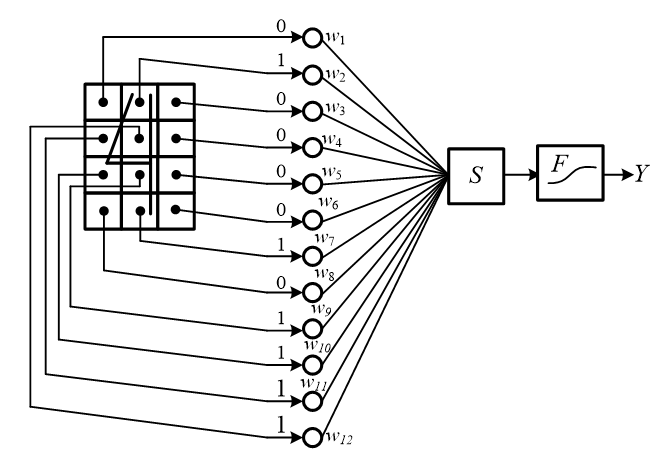
\includegraphics[scale=0.5]{images/lec03-binary.png}
	\end{figure}
\end{frame}

\begin{frame}[t]{Задача бинарной классификации}
	\begin{itemize}
		\item задаются \textbf{два класса}: 1 (положительный класс), -1 (отрицательный класс);
		\item рассчитывается \textbf{чистый вход} - линейная комбинация весов и входных значений $z=w_1\cdot x_1+...+w_m\cdot x_m$;
	\end{itemize}
	\begin{figure}[h]
		\centering
		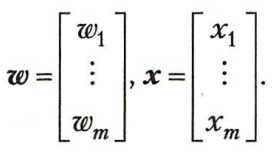
\includegraphics[scale=0.5]{images/lec03-pic02.png}
	\end{figure}
	\begin{itemize}
		\item определяется передаточная функцию (функция активации) $\phi(z)$;
		\item в алгоритме персептрона функция активации - это простая ступенчатая функция Хевисайда;
	\end{itemize}
	\begin{figure}[h]
		\centering
		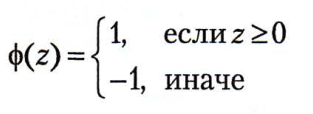
\includegraphics[scale=0.4]{images/lec03-pic03.png}
	\end{figure}
\end{frame}

\begin{frame}[t]
	\begin{itemize}
		\item активация отдельно взятого образца $x^{(i)}$, т. е. выход из $\phi(z)$, превышает заданный порог, то мы распознаем класс 1, в противном случае - класс -1;
		\item порог учитывается так: $w_0 = -\theta, x_0 = -1$;
	\end{itemize}
	\begin{figure}[h]
		\centering
		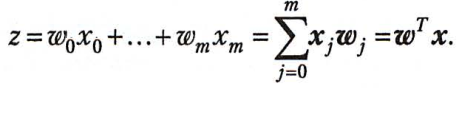
\includegraphics[scale=0.4]{images/lec03-pic04.png}
	\end{figure}
	\begin{figure}[h]
		\centering
		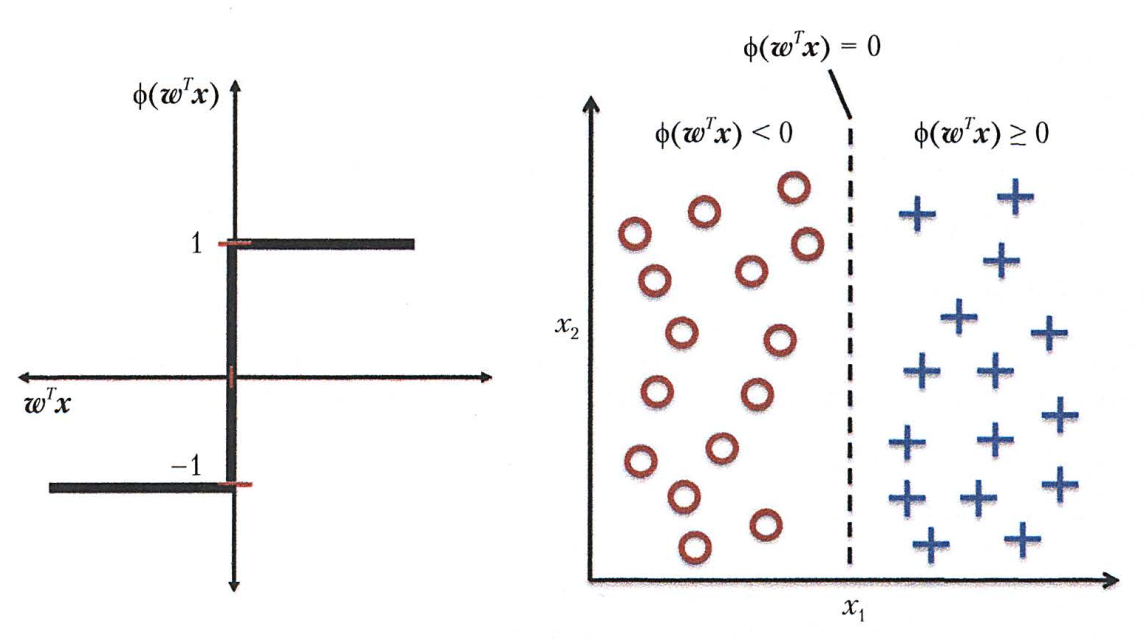
\includegraphics[scale=0.25]{images/lec03-pic05.png}
	\end{figure}
\end{frame}

\begin{frame}[t]{Обучение персептрона}
	\linespread{1.0}
	Идея, лежащая в основе обучение персептронной модели Розенблатта:
	\begin{enumerate}
		\item В процессе обучения корректируются весовые коэффициенты таким образом, чтобы ошибка классификации для всех цифр была равна нулю или меньше заданной погрешности. 
		\item Обучение происходит с использованием обучающих примеров, подобно обучению маленьких детей словам или буквам. 
		\item Каждый пример предъявляется распознающему устройству неоднократно и при правильном распознавании типа цифры веса не меняются, а при наличии ошибки корректируются, пока не будет достигнута безошибочная классификация.		
	\end{enumerate}
\end{frame}

\begin{frame}[t]{Схема обучения}
	\begin{figure}[h]
		\centering
		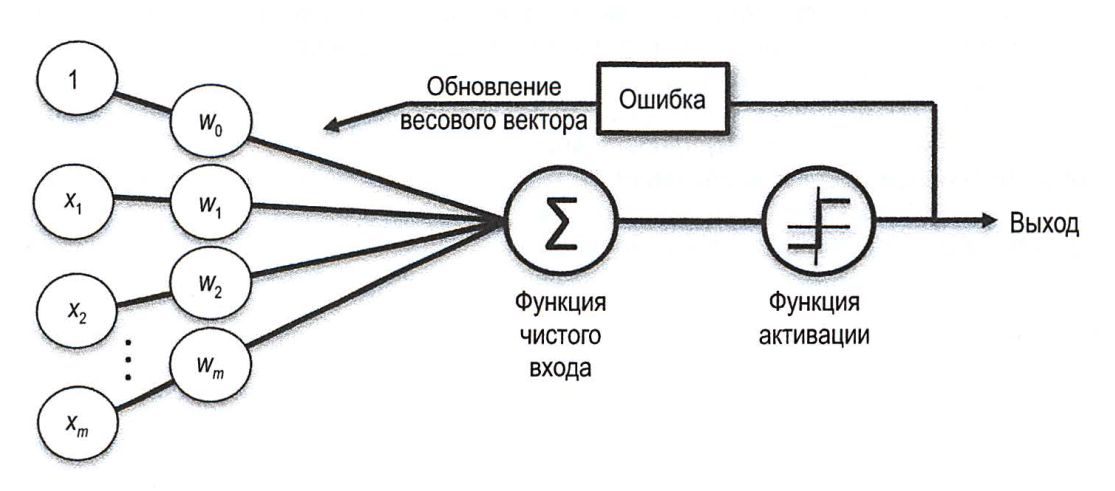
\includegraphics[scale=0.4]{images/lec03-pic09.png}
	\end{figure}
\end{frame}

\begin{frame}[t]{Обучение персептрона}
	Алгоритм обучения персептронной модели Розенблатта:
	\begin{enumerate}
		\item инициализировать веса нулями либо малыми случайными числами;
		\item для каждого тренировочного образца $x^{(i)}$ выполнить следующие шаги:
		\begin{itemize}
			\item вычислить выходное значение $\hat{y}$;
			\item обновить веса.
		\end{itemize}
	\end{enumerate}
	\textbf{Выходное значение} - метка класса, идентифицированная единичной ступенчатой функцией.
	\[\omega_j := \omega_j + \Delta\omega_j\]
	Значение $\Delta\dot\omega_j$ вычисляется правилом обучения персептрона:
	\[\Delta\omega_j := \eta(y^{(i)} - \hat{y}^{(i)})x^{(i)}_j \]
	\begin{itemize}
		\item $\eta$ - темп обучения (константа 0.0..1.0);
		\item $y^{(i)}$ - истинная метка класса i-го тренировочного образца;
		\item $\hat{y}^{(i)}$ - идентифицированная метка класса. 
	\end{itemize}
\end{frame}

\begin{frame}[t]
	Персептрон правильно распознает метку класса, веса остаются неизменными:
	\begin{figure}[h]
		\centering
		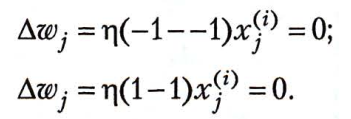
\includegraphics[scale=0.5]{images/lec03-pic06.png}
	\end{figure}
	В случае неправильного распознавания веса продвигаются в направлении соответственно 	положительного или отрицательного целевого класса:
	\begin{figure}[h]
		\centering
		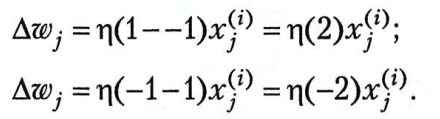
\includegraphics[scale=0.5]{images/lec03-pic07.png}
	\end{figure}
\end{frame}

\begin{frame}[t]
	\linespread{1.0}
	Замечания о сходимости:
	\begin{enumerate}
		\item сходимость персептрона гарантируется, только если эти два класса линейно разделимы и темп обучения достаточно небольшой. 
		\item если эти два класса не могут быть разделены линейной границей решения, необходимо установить максимальное число проходов по тренировочному набору данных (эпох) и/или порог на допустимое число случаев ошибочной классификации, иначе обновление весов будет продолжаться бесконечно.
	\end{enumerate}
	\begin{figure}[h]
		\centering
		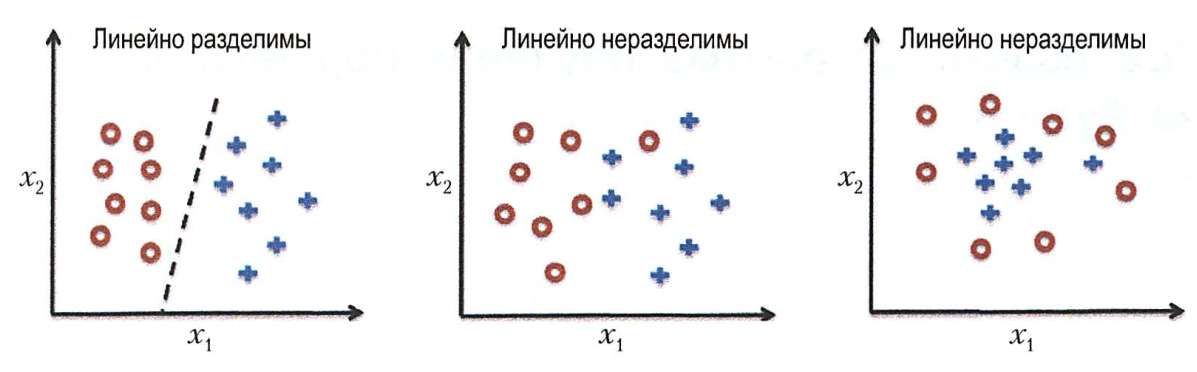
\includegraphics[scale=0.35]{images/lec03-pic08.png}
	\end{figure}
\end{frame}

\begin{frame}[t]
	\linespread{1.0}
	Всегда ли алгоритм обучения персептрона приводит к желаемому результату?
	
	\begin{block}{Теорема сходимости персептрона}
		если существует множество значений весов, которые обеспечивают конкретное различение образов, то в конечном итоге алгоритм обучения персептрона приводит либо к этому множеству, либо к эквивалентному множеству, такому, что данное различение образов будет достигнуто.	
	\end{block}
	\begin{figure}[h]
		\centering
		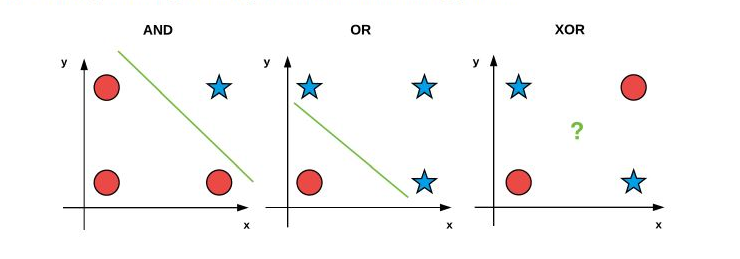
\includegraphics[scale=0.6]{images/lec03-xor.png}
	\end{figure}	
\end{frame}

%\subsection{Аддитивные линейные нейроны и сходимость обучения}

\begin{frame}[t]
	\textbf{ADALINE} -- ADAptive LInear NEuron, адаптивный линейный нейрон.
	\begin{itemize}
		\item для обновления весов используется линейная функция активации $\phi(\omega^T x) = \omega^Tx$, а не единичная ступенчатая, как в персептроне;
		\item с целью распознавания меток классов используется квантизатор, аналогичный встречавшейся ранее единичной ступенчатой функции.
	\end{itemize}
	\begin{figure}[h]
		\centering
		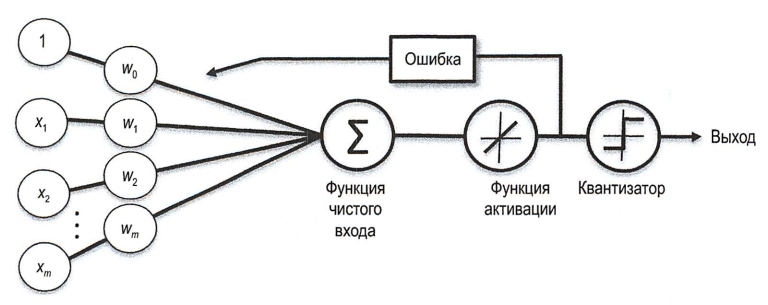
\includegraphics[scale=0.4]{images/lec03-pic19.png}
	\end{figure}
	Б. Видроу и др., Адаптивный нейрон <<Adaliпe>> с использованием химических <<мемисторов>>~- Numbeг Technical Repoгt Stanfoгd Electгon Labs, Стэнфорд, Калифорния, 1960
\end{frame}

\begin{frame}[t]
	\textit{Ключевая составляющая алгоритмов машинного обучения с учителем}: задание целевой функции, которая подлежит оптимизации во время процесса обучения.
	~
	Пример среднеквадратической ошибки распознавания цифр:
	\[J(W)=1/2 \sum_{k=0}^{9} (y_k(X_k, W)-d_k)^2\]
	\begin{itemize}
		\item $X_k={x_{k,i}, i=1..12}$ -- вектор входных сигналов, для каждой цифры~-- своя битовая строка;
		\item $W_k={w_{i}, i=1..12}$ -- весовые коэффициенты, значения которых должны быть найдены в процессе обучения;
		\item $y_k(X_k, W)$	-- сигнал на выходе нейрона при подаче на его вход $k$-й цифры и значениях весовых коэффициентов;
		\item $d_k$ -- заданное значение выходного сигнала для $k$-й цифры (если цифра четная, то $d_k=1$, если цифра нечетная, то $d_k=0$);		
		\item $e_k=|y_k(X_k, W)-d_k|$ -- ошибка распознавания k-й цифры;
	\end{itemize}
\end{frame}

\begin{frame}[t]
	\begin{block}{Градиент}
		вектор, состоящий из частных производных анализируемой функции по ее аргументам.	
	\end{block}
	\begin{itemize}
		\item задает направление наискорейшего возрастания функции в некоторой точке; 				\item при поиске минимума функции необходимо двигаться в направлении, противоположном вектору градиента, или вдоль вектора, составляющего тупой угол с вектором градиента.
	\end{itemize}
	\begin{figure}[h]
		\centering
		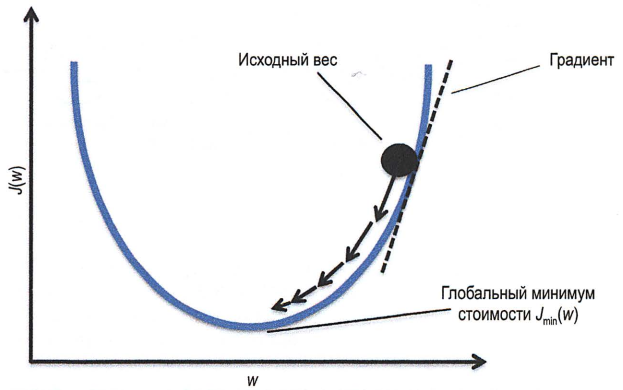
\includegraphics[scale=0.4]{images/lec03-pic21.png}
	\end{figure}
\end{frame}

\begin{frame}[t]
	Обновление веса на основе градиентного спуска путем выполнения шага в противоположную сторону от градиента целевой функции:
	\[w_i(t+1)=w_i(t)-\eta\cdot G_i\]
	где
	\begin{itemize}
		\item $w_i(t+1)$ -- новое значение весовых коэффициентов; 
		\item $w_i(t)$ -- старое значение весовых коэффициентов;		
		\item $\eta$ -- скорость обучения;				
		\item $G_i = \partial J/\partial w_i$ -- вектор градиента.						
	\end{itemize}	
\end{frame}

\begin{frame}[t]
	Для нейрона, распознающего цифры, вектор градиента будет иметь вид: 
	\[G_i = \frac{\partial J}{\partial y_k} \frac{\partial y_k}{\partial w_i} 
	      = \frac{1}{2}\cdot 2\cdot (y_k-d_k)\frac{\partial \sum_{i=1}^{12}x_{k_i}w_i}{\delta w_i}
		  = e_k\cdot x_{k,i}	 
	\]
	где
	\begin{itemize}
		\item $i$ -- номер входного сигнала; 
		\item $e_k$ -- ошибка при предъявлении $k$-го примера ($k$-ой цифры);		
	\end{itemize}
	Формула подстройки весовых коэффициентов при предъявлении $k$-го примера:
	\[w_i(t+1)=w_i(t)-\eta\cdot e\cdot x_i\]	
	Подстройка порогового значения нейрона:
	\[w_0(t+1)=w_0(t)-\eta\cdot e\]
	Первоначально весовым коэффициентам даются произвольные значения с помощью датчика случайных чисел.
\end{frame}

\begin{frame}[t]
	\begin{figure}[h]
		\centering
		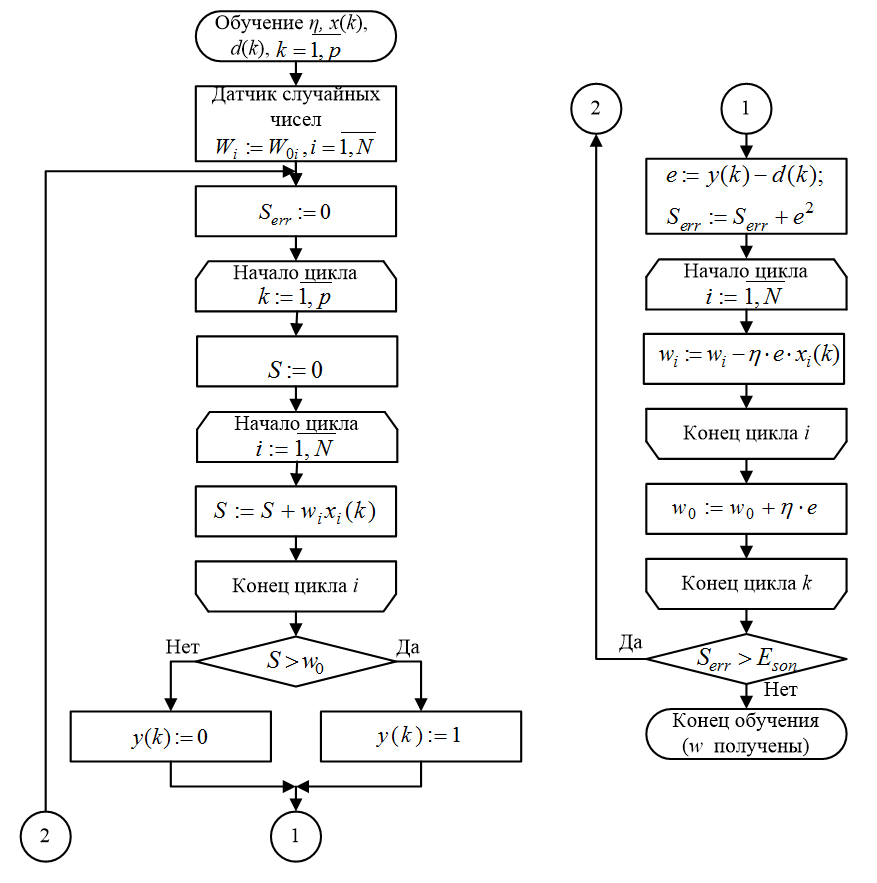
\includegraphics[scale=0.35]{images/lec03-alg.png}
		\caption{Схема алгоритма подстройки весов}
	\end{figure}
\end{frame}

\begin{frame}[t]
	\begin{figure}[h]
		\centering
		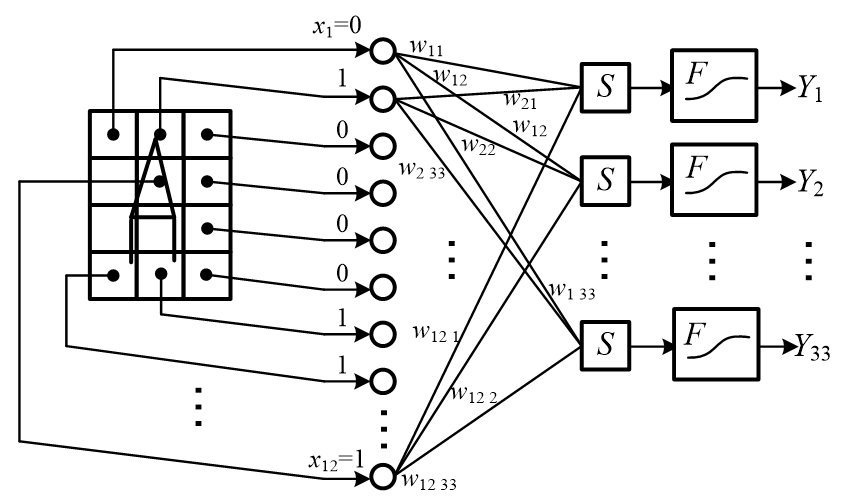
\includegraphics[scale=0.5]{images/lec03-letters.png}
		\caption{Схема нейрона для распознавания букв}
	\end{figure}
\end{frame}

\begin{frame}[t]
	\begin{figure}[h]
		\centering
		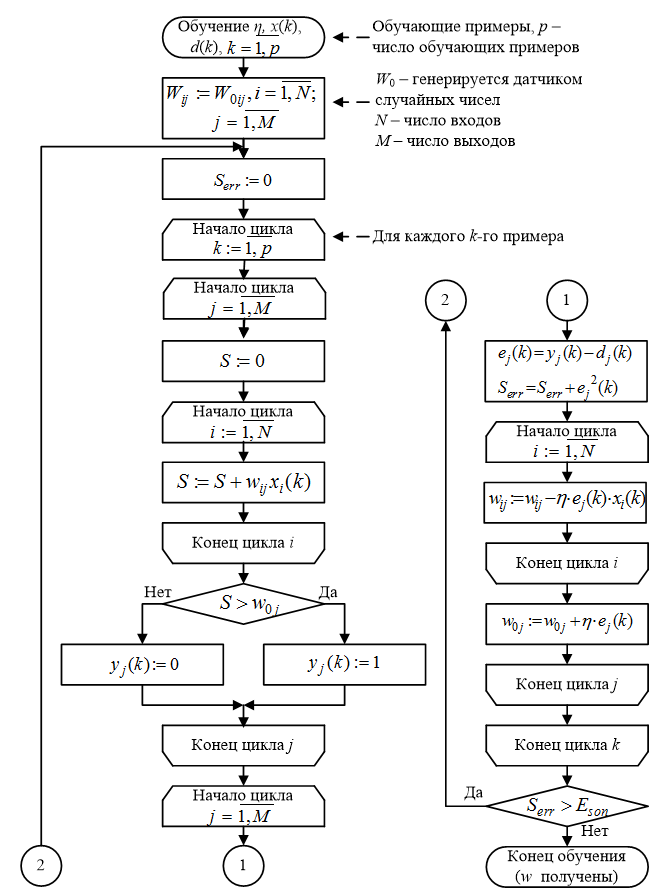
\includegraphics[scale=0.35]{images/lec03-alg-letters.png}
		\caption{Схема алгоритма подстройки весов}
	\end{figure}
\end{frame}

\begin{frame}[t]
	\textbf{Сигмоида} -- нелинейная функция активации (Уидроу,Хофф): 
	\[ y = f(S) = \frac{1}{(1+e^{-\alpha S})} \]
	где
	\begin{itemize}
		\item $\alpha$ -- положительная константа, от значения которой зависит крутизна сигмоиды;		
		\item $f(S)$ -- обозначение произвольной активационной функции.		
	\end{itemize}
	\begin{figure}[h]
		\centering
		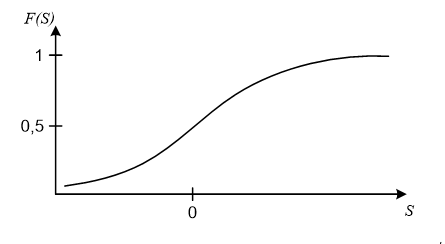
\includegraphics[scale=0.5]{images/lec03-sigmoid.png}
	\end{figure}
	\begin{itemize}
		\item выходное значение нейрона лежит в диапазоне $[0,1]$. 
		\item дифференцируема на всей оси абсцисс; 
		\item усиливает малые сигналы лучше, чем большие -- предотвращает насыщение от больших сигналов.
	\end{itemize}	
\end{frame}

\begin{frame}[t]{Настройка весов}
	Целевая функция:
	\[J=1/2 \sum_{k=1}^{33} (\overrightarrow{y_k}(X_k, W)-\overrightarrow{d_k})^2\]
	Подстройка весовых коэффициентов для $k$-го примера:
	\[w_{ij}(t+1)=w_{ij}(t)-\eta\cdot e_j\cdot f'(S_j)\cdot x_i, i=1..m, j=1..n\]	
	Если $f(S)$ -- сигмоида, то ее производная
	\[f'(S)=((1+e^{\alpha S_j})^{-1})'=f(S)(1-f(S))\]
	Тогда формула подстройки весов примет вид:
	\[w_{ij}(t+1)=w_{ij}(t)-\eta\cdot e_j\cdot y_i\cdot (1-y_i)\cdot x_i, i=1..m, j=1..n\]		
	где $e_j=y_j-d_j$.
\end{frame}

\begin{frame}[t]{Ограниченность однослойного персептрона}
	\begin{itemize}
		\item персептроны в принципе не способны решать многие простые задачи (<<Персептроны>> М. Минский и С. Пайперт);
		\item предложено усложнить структуру персептронов, использовать два слоя нейронов: 
	\end{itemize}		
	\begin{figure}[h]
		\centering
		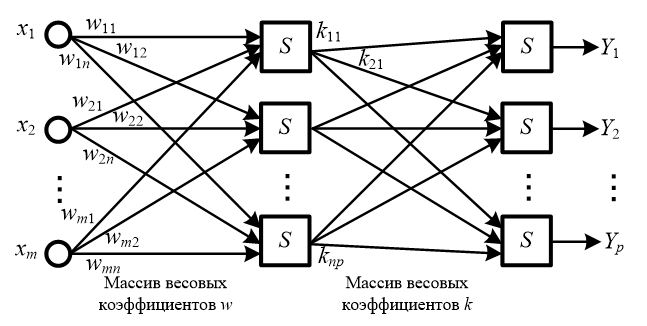
\includegraphics[scale=0.5]{images/lec03-twolayer.png}
	\end{figure}		
	\begin{itemize}	
		\item Многослойные нейронные сети расширяют класс задач, решаемых персептронами. 
	\end{itemize}
\end{frame}

\begin{frame}[t]{Дискретный динамический процесс как модель нейронной сети}
	Рассмотрим постановку задачи подстройки весовых коэффициентов многослойной нейронной сети как задачу оптимального управления дискретным динамическим процессом.
	~
	Пусть 
	\begin{itemize}
		\item $x(n)={x_0(n), x_1(n),...,x_{m_n}(n)} $ -- сигнал на входе n-ого слоя сети;
		\item $m_n$ -- число нейронов в слое $n$;
		\item $x(n) $ -- вектор-строка;
		\item $x^T(n) $ -- вектор-столбец;
		\item $x_0(n)=1$;
		\item $u(n)=W(n)$ -- матрица весовых коэффициентов n-го слоя сети размером $m_{n-1}:m_n$;			
		\item $x(0)$ -- сигналы, подаваемые на вход нейронной сети;
		\item $(x_k(0)=a^k; x^k(N)=d^k), k=1,2,...,P $ -- обучающие примеры: при k-м входном сигнале $x_k(0)=a^k$ на выходе сети необходимо обеспечить сигнал $x^k(N)=d^k$ путем выбора весовых коэффициентов $W$.
	\end{itemize}
\end{frame}

\begin{frame}[t]{Задача настройки нейронной сети}
	Найти такие значения оптимального управления $u(n)=W(n), n=1,2,...,N$, при которых будут выполнены ограничения:
	\[
	x(0)=a; x(n)=f^n(S(n))=f^n((x(n-1)\cdot W(n)))
	\]
	где 
	\begin{itemize}
		\item $f^n(..)$ - активационная функция;
		\item $S(n)=x(n-1)\cdot W(n)$ - вектор сумм взвешенных сигналов для n-го слоя нейронной сети;
		\item $n=1,2,...,N$.
	\end{itemize}
	Критерий качества процесса: 
	\[
	\text{min }\Phi(x(N))=\text{min } \sum_{k=1}^P (x^k(N)-d^k)^2.
	\]
	
	Система называется \textbf{прямой системой уравнений}, используется для получения сигнала на выходе нейронной сети при заданных значениях весовых коэффициентов $W$ и известном входном сигнале.
\end{frame}

\begin{frame}[t]
	\begin{block}{\textbf{Сопряженная} (двойственная система)}
		описывает процесс, который называют <<обратным распространением ошибки>>.
	\end{block}	
	\[p(N)=\frac{\partial \Phi(x(N))}{\partial x(N)};\]
	\[p(n-1) = \left[\frac{\partial f(x(n-1), u(n))}{\partial x(n-1)}\right]^T\cdot p(n), n=N,...,1\]
	где 
	\begin{itemize}
		\item $p(n)={p_1(n),...,p_{mn}(n)}$;
		\item $\frac{\partial f(x,u)}{\partial x} = \left[\frac{\partial f_i(x,u)}{\partial x_j}\right], i=1..m_n, j=1..m_{n-1}$
		\item $m_{n-1}, m_n$ -- число нейронов в слое $n-1$ и в слое $n$;
	\end{itemize}
	Функция Гамильтона:
	\[H(p(n),x(n-1),W(n))=(p(n), f^n(x(n-1)\cdot W(n)))\]
	При фиксированных $p$ и $x$ функция Гамильтона становится функцией только управляющего воздействия $W(n)$.
\end{frame}

\linespread{1.0}
\begin{frame}[t]{Алгоритм подстройки весов многослойной нейросети}
	\begin{enumerate}
		\item задание произвольных значений весовых коэффициентов для всех слоев;
		\item расчет по формулам сигналов $x(n), n=1,2,...,N$ на выходе каждого слоя нейронов;
		\item расчет по формулам сопряженного вектора $p(n), n = N, N–1,...1$, по значению которого можно определить слой, наиболее влияющий на критерий оптимальности;
		\item вычисление для каждого слоя функции Гамильтона;
		\item для каждого слоя определение направления изменения значений весовых коэффициентов в сторону уменьшения функции Гамильтона одним из известных методов (градиентным, методом Ньютона и т.д.);
		\item определение длины шага и нового управления;
		\item оценка близости полученного решения к оптимальному решению.
	\end{enumerate}
\end{frame}

\begin{frame}[t]
	Всегда ли можно построить нейросеть, выполняющую преобразование, заданное любой обучающей выборкой?
	\begin{block}{Теорема}
		\begin{itemize}		
			\item Для любого множества пар отличных между собой входных и выходных векторов произвольной размерности $(X_q, D_q), q = 1,...,P$ существует двухслойный персептрон с сигмоидальными активационными функциями и с конечным числом нейронов, который для каждого входного вектора $X_q$ формирует соответствующий ему  выходной вектор $D_q$. 
		\end{itemize}	
	\end{block}
	Количество нейронов в скрытых слоях персептрона:
	\[
		\frac{N_y\cdot P}{1+log_2P} \leq N_w \leq N_y(P/N_x+1)\cdot (N_x+N_y+1)+N_y
	\]
	где
	\begin{itemize}		
		\item $N_y$ -- размерность выходного сигнала; 
		\item $P$ -- число элементов обучающей выборки; 
		\item $N_w$ -- необходимое число синаптических весов; 
		\item $N_x$ -- размерность входного сигнала.
	\end{itemize}	
\end{frame}

\begin{frame}[t]{Предобработка обучающих примеров}
	Исключение незначимых параметров:
	\begin{itemize}
		\item путем анализа значений весовых коэффициентов входных нейронов; 
		\item путем возмущения значений входных параметров и анализа реакции сети на эти возмущения.
	\end{itemize}
	Предобработка обучающих примеров:
	\begin{itemize}
		\item кодирование в числовом виде; 
		\item выравнивание диапазонов изменения величин в интервалы [0,1] или [-1, 1].
		\[
		\tilde{x_n} = \frac{x_n-x_{n\text{min}}}{x_{n\text{max}-x_{n\text{min}}}}\cdot (b-a)+a
		\]
	\end{itemize}
	где
	\begin{itemize}
		\item $\tilde{x_n}$ и $x_n$ -- значения исходного и масштабированного n-го параметра предметной области, подаваемого на n-й входной нейрон сети;
		\item $x_{n\text{max}}, x_{n\text{min}}$ -- реальный диапазон изменения n-го параметра;
		\item $[a,b]$ -- приемлемый диапазон изменения входных сигналов.
	\end{itemize}
	Выходные сигналы персептрона должны быть также закодированы в приемлемой форме и масштабированы.
\end{frame}

\begin{frame}[t]
	При проектировании персептронов существует проблема выбора необходимого числа нейронов: 
	\begin{itemize}
		\item число нейронов входного слоя персептрона должно совпадать с размерностью вектора входных параметров X, который определен условиями решаемой задачи;
		\item число нейронов выходного слоя должно совпадать с размерностью выходного вектора Y, что также определено условиями задачи. 
		\item число нейронов в скрытых слоях может быть приближенно оценено по следующим формулам, однако его желательно оптимизировать для каждой конкретной задачи.
	\end{itemize}
	Число нейронов скрытого слоя двухслойного персептрона:
	\[
		N = \frac{N_w}{N_x+N_y}
	\]	
	\begin{itemize}
		\item Строгой теории выбора оптимального числа скрытых слоев персептронов пока нет. 
		\item На практике же чаще всего используются персептроны, имеющие один или два скрытых слоя, причем число нейронов в скрытых слоях обычно колеблется от $N_x$ до $3N_x$.	
	\end{itemize}
\end{frame}

\linespread{1.0}
\begin{frame}[t]
	При проектировании персептрона необходимо понимать, что персептрон должен:  
	\begin{itemize}
		\item правильно реагировать на обучающие примеры;
		\item уметь обобщать приобретенные знания, т.е. правильно реагировать на  случаи, которых в обучающей выборке не было.
	\end{itemize}	 
	Чтобы оценить способность сети к обобщению, помимо обучающей выборки примеров $(X;D)$ в рассмотрение вводят некоторое количество тестовых примеров $(X_T;D_T)$, которые относятся к той же предметной области, но в процессе обучения не участвуют.	
	\begin{block}{Погрешность обучения}
	среднеквадратичная погрешность персептрона, вычисленная на обучающей выборке $(X;D)$.
	\end{block}
	\begin{block}{Погрешность обобщения}
	среднеквадратичная погрешность персептрона, вычисленная на тестовой выборке $(X_t;D_t)$.
	\end{block}	 
\end{frame}

\begin{frame}[t]{Переобучение}
При увеличении числа нейронов внутренних слоев персептрона N:
	\begin{itemize}
	\item погрешность обучения обычно падает;
	\item погрешность обобщения сначала падает, а затем, начиная с некоторого оптимального значения $N = N_0$, возрастает.
	\end{itemize}
	\begin{block}{Переобучение}
	свойство нейросети терять способность к обобщению при чрезмерном увеличении числа ее синаптических связей.
	\end{block}	
	
	\textbf{Проблема обучения персептронов}: 	поверхность функции ошибок обычно имеет очень сложную форму с множеством локальных минимумов. 
	\begin{itemize}{}
	\item актуальным является развитие методов глобальной оптимизации;
	\item наиболее успешным признается идея генетических алгоритмов для подстройки весов.
	\end{itemize}
\end{frame}

\end{document}
